% Options for packages loaded elsewhere
\PassOptionsToPackage{unicode}{hyperref}
\PassOptionsToPackage{hyphens}{url}
%
\documentclass[
  ignorenonframetext,
  aspectratio=169]{beamer}
\usepackage{pgfpages}
\setbeamertemplate{caption}[numbered]
\setbeamertemplate{caption label separator}{: }
\setbeamercolor{caption name}{fg=normal text.fg}
\beamertemplatenavigationsymbolsempty
% Prevent slide breaks in the middle of a paragraph
\widowpenalties 1 10000
\raggedbottom
\setbeamertemplate{part page}{
  \centering
  \begin{beamercolorbox}[sep=16pt,center]{part title}
    \usebeamerfont{part title}\insertpart\par
  \end{beamercolorbox}
}
\setbeamertemplate{section page}{
  \centering
  \begin{beamercolorbox}[sep=12pt,center]{part title}
    \usebeamerfont{section title}\insertsection\par
  \end{beamercolorbox}
}
\setbeamertemplate{subsection page}{
  \centering
  \begin{beamercolorbox}[sep=8pt,center]{part title}
    \usebeamerfont{subsection title}\insertsubsection\par
  \end{beamercolorbox}
}
\AtBeginPart{
  \frame{\partpage}
}
\AtBeginSection{
  \ifbibliography
  \else
    \frame{\sectionpage}
  \fi
}
\AtBeginSubsection{
  \frame{\subsectionpage}
}
\usepackage{lmodern}
\usepackage{amssymb,amsmath}
\usepackage{ifxetex,ifluatex}
\ifnum 0\ifxetex 1\fi\ifluatex 1\fi=0 % if pdftex
  \usepackage[T1]{fontenc}
  \usepackage[utf8]{inputenc}
  \usepackage{textcomp} % provide euro and other symbols
\else % if luatex or xetex
  \usepackage{unicode-math}
  \defaultfontfeatures{Scale=MatchLowercase}
  \defaultfontfeatures[\rmfamily]{Ligatures=TeX,Scale=1}
\fi
\usetheme[]{Frankfurt}
\usecolortheme{beaver}
% Use upquote if available, for straight quotes in verbatim environments
\IfFileExists{upquote.sty}{\usepackage{upquote}}{}
\IfFileExists{microtype.sty}{% use microtype if available
  \usepackage[]{microtype}
  \UseMicrotypeSet[protrusion]{basicmath} % disable protrusion for tt fonts
}{}
\makeatletter
\@ifundefined{KOMAClassName}{% if non-KOMA class
  \IfFileExists{parskip.sty}{%
    \usepackage{parskip}
  }{% else
    \setlength{\parindent}{0pt}
    \setlength{\parskip}{6pt plus 2pt minus 1pt}}
}{% if KOMA class
  \KOMAoptions{parskip=half}}
\makeatother
\usepackage{xcolor}
\IfFileExists{xurl.sty}{\usepackage{xurl}}{} % add URL line breaks if available
\IfFileExists{bookmark.sty}{\usepackage{bookmark}}{\usepackage{hyperref}}
\hypersetup{
  pdftitle={Genetic engineering in plants},
  pdfauthor={Deependra Dhakal},
  hidelinks,
  pdfcreator={LaTeX via pandoc}}
\urlstyle{same} % disable monospaced font for URLs
\newif\ifbibliography
\setlength{\emergencystretch}{3em} % prevent overfull lines
\providecommand{\tightlist}{%
  \setlength{\itemsep}{0pt}\setlength{\parskip}{0pt}}
\setcounter{secnumdepth}{-\maxdimen} % remove section numbering
% % set background image if you will
% \usebackgroundtemplate%
% {%
%     \includegraphics[width=\paperwidth,height=\paperheight]{02-dna_modification_background_dna_helix.jpg}%
% }

% % set caption font size
% % note that beamer presentation native captions have their own configs
% \usepackage{caption}
% \captionsetup{font=footnotesize}

% this font option is amenable for beamer
\setbeamerfont{caption}{size=\tiny}

% some beamer themes naturally might not support navigation symbols
% \setbeamertemplate{navigation symbols}{} % remove navigation symbols

\setbeamertemplate{footline}[page number] % insert page number in footline

% \setbeamertemplate{navigation symbols}{slide} % insert slide indication in navigation
% \setbeamertemplate{navigation symbols}{frame} % insert frame indication in navigation
% \setbeamertemplate{navigation symbols}{section} % insert section indication in navigation
% \setbeamertemplate{navigation symbols}{subsection} % insert subsection indication in navigation

% \AtBeginSubsection{} % supress subsection display
\newlength{\cslhangindent}
\setlength{\cslhangindent}{1.5em}
\newenvironment{cslreferences}%
  {\setlength{\parindent}{0pt}%
  \everypar{\setlength{\hangindent}{\cslhangindent}}\ignorespaces}%
  {\par}

\title{Genetic engineering in plants}
\author{Deependra Dhakal}
\date{Academic year 2022-2023}
\institute{CNRM, Tikapur \and Agriculture and Forestry University}

\begin{document}
\frame{\titlepage}

\begin{frame}[allowframebreaks]
  \tableofcontents[hideallsubsections]
\end{frame}
\hypertarget{overview}{%
\section{Overview}\label{overview}}

\begin{frame}{Rationale}
\protect\hypertarget{rationale}{}
\begin{itemize}
\tightlist
\item
  Finding desirable genes can be difficult because multiple interacting
  genes usually control certain beneficial traits.
\item
  So far, most successful genetic engineering of plants has relied on
  inserting one or a few genes that supply simple, yet useful,
  properties.
\item
  ``Gene technology'' encompasses the spectrum of methods used to
  achieve new combinations of hereditary material.
\item
  If recombinant DNA is introduced into a living cell and stably
  incorporated, integrated, into the genome (generally into the nuclear
  genome, but also in eukaryotic plants into the plastome, as well as
  other sites), then a genetically modified cell/organism is produced.
\item
  Independent of whether it is a gene from the same species or from
  another species, a hybrid gene (a gene made of sections of genes from
  different organisms), or a synthetic gene, they are called transgenic
  organisms or genetically modified organisms (GMOs)
\end{itemize}
\end{frame}

\begin{frame}{Genetically modified organism}
\protect\hypertarget{genetically-modified-organism}{}
\begin{itemize}
\tightlist
\item
  A task force of the Codex Alimentarius Commission, a U.N. agency
  responsible for an international code for food standardization, has
  advanced the following language to standardize the labeling of foods
  derived from GMOs for purposes of international commerce:
\end{itemize}

\begin{block}{GMO}
Genetically modified/engineered organism means an organism in which the genetic material has been changed through gene technology in a way that does not occur naturally by multiplication and/or any natural recombination.
\end{block}
\end{frame}

\hypertarget{agrobacterium-mediated-transformation}{%
\section{Agrobacterium mediated
transformation}\label{agrobacterium-mediated-transformation}}

\begin{frame}{Background}
\protect\hypertarget{background}{}
\begin{itemize}
\tightlist
\item
  Plants suffer tumors!
\item
  Commonly due to bacteria ( \emph{Agrobacterium tumefaciens})
  containing plasmid DNA (Ti)
\item
  Specific segment of the plasmid DNA is transferred to the host plant
\item
  Modern Ti plasmids are disarmed to suit genetic engineering
\item
  Binary vectors: A transfer DNA (T-DNA) binary system is a pair of
  plasmids consisting of a T-DNA binary vector and a vir helper
  plasmid\footnote<.->{See
    \url{https://en.wikipedia.org/wiki/Transfer_DNA_binary_system}}.
\end{itemize}
\end{frame}

\begin{frame}{Background (Infected and non-infected plants)}
\protect\hypertarget{background-infected-and-non-infected-plants}{}
\begin{columns}[T,onlytextwidth]
  \column{0.5\textwidth}

\begin{figure}
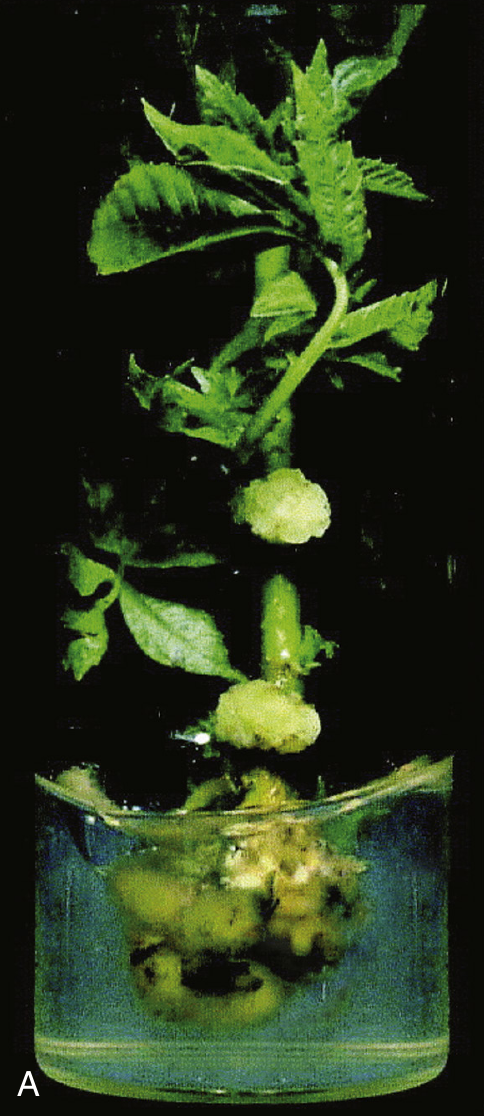
\includegraphics[width=0.4\linewidth]{../images/agrobacterium_gall_a} \caption{Crown gall tumors are caused by Agrobacterium tumefaciens}\label{fig:agrobacterium-gall1}
\end{figure}

  \column{0.5\textwidth}

\begin{figure}
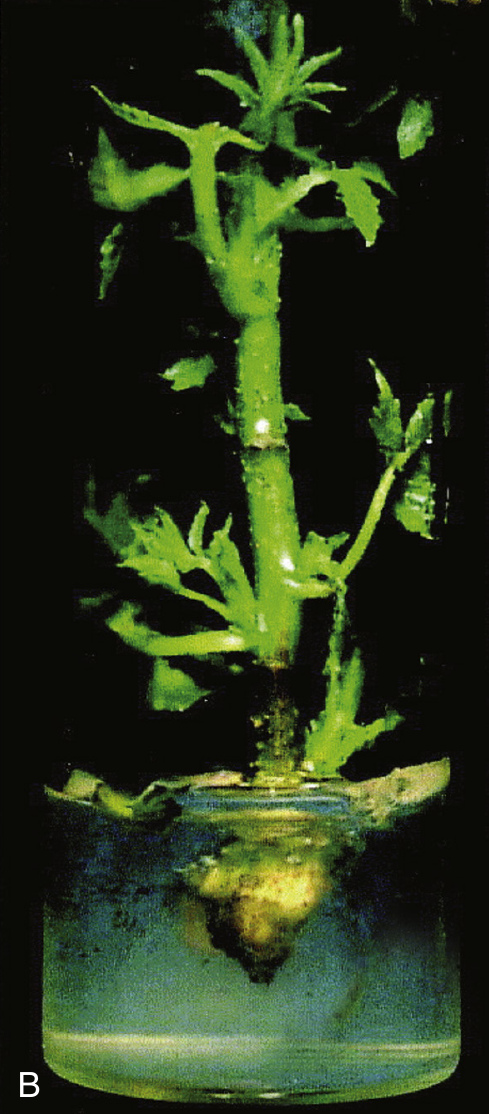
\includegraphics[width=0.4\linewidth]{../images/agrobacterium_gall_b} \caption{But plants expressing inhibitors of key proteins for Agrobacterium infection do not develop any tumors (B)\newline Crown gall disease in walnut (Juglans regia L.)}\label{fig:agrobacterium-gall2}
\end{figure}
    
\end{columns}
\end{frame}

\begin{frame}{Ti-plasmid structure}
\protect\hypertarget{ti-plasmid-structure}{}
\begin{figure}
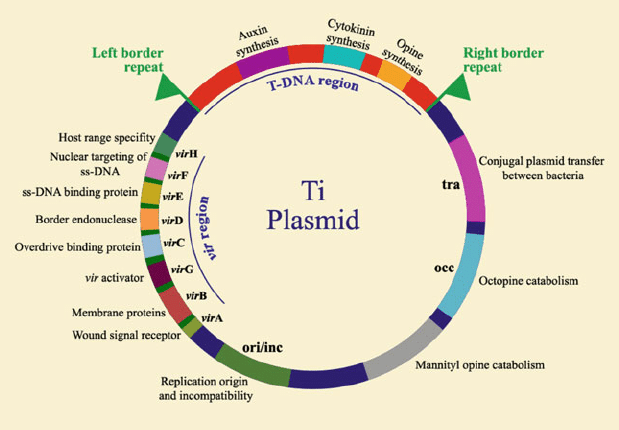
\includegraphics[width=0.5\linewidth]{../images/Ti_plasmid} \caption{The structure of the Ti plasmid}\label{fig:ti-plasmid}
\end{figure}
\end{frame}

\begin{frame}{Ti-plasmid structure}
\protect\hypertarget{ti-plasmid-structure-1}{}
\begin{itemize}
\tightlist
\item
  Genes in the virulence region are grouped into the operons virABCDEFG,
  which code for the enzymes responsible for mediating conjugative
  transfer of T-DNA to plant cells (Stachel and Nester 1986).

  \begin{itemize}
  \tightlist
  \item
    virA codes for a receptor which reacts to the presence of phenolic
    compounds such as acetosyringone, syringealdehyde or acetovanillone
    which leak out of damaged plant tissues.
  \item
    virB encodes proteins which produce a pore/pilus-like structure.
  \item
    virC binds the overdrive sequence.
  \item
    virD1 and virD2 produce endonucleases which target the direct repeat
    borders of the T-DNA segment; virD4 is the coupling protein.
  \item
    virE binds to T-strand protecting it from nuclease attack, and
    intercalates with lipids to form channels in the plant membranes
    through which the T-complex passes, beginning with the right border.
  \item
    virG activates vir-gene expression after binding to a consensus
    sequence, once it has been phosphorylated by virA.
  \end{itemize}
\end{itemize}
\end{frame}

\begin{frame}{Infection by Ti-plasmid}
\protect\hypertarget{infection-by-ti-plasmid}{}
\begin{itemize}
\tightlist
\item
  Wounded plant tissues produce special compound called
  \emph{acetosyringone}
\item
  The plant inducers (Phenolic compounds) activate expression of the
  virulence genes on the Ti plasmid. This is under control of a
  two-component regulatory system.
\item
  This initiates the T-DNA transfer machinery
\item
  Plants may employ defense mechanism to prevent the infection and T-DNA
  transfer
\end{itemize}
\end{frame}

\begin{frame}{Infection by Ti-plasmid}
\protect\hypertarget{infection-by-ti-plasmid-1}{}
\begin{itemize}[<+->]
\tightlist
\item
  \alert<1>{Once the vir genes are activated, the T-DNA is processed for transport to the target plant cell.}
\item
  \emph{VirA} transfers the phosphate to the DNA-binding protein,
  \emph{VirG}, which activates transcription of the vir genes of the Ti
  plasmid.
\item
  Two of the gene products ( \emph{VirD1} and \emph{VirD2}) clip the
  T-DNA borders to form a single-stranded immature T-complex.
\item
  \emph{VirD2} then attaches to the \(5^\prime\) end of the T-DNA, and
  bacterial helicases unwind the T-DNA from the plasmid.
\item
  The single-stranded gap on the plasmid is repaired, and the T-DNA is
  coated with \emph{VirE2} protein to give a hollow cylindrical filament
  with a coiled structure.
\end{itemize}
\end{frame}

\begin{frame}{Infection by Ti-plasmid}
\protect\hypertarget{infection-by-ti-plasmid-2}{}
\begin{itemize}
\tightlist
\item
  Yet additional vir gene products bind to the T-DNA to act as
  navigators or signals to direct the mature DNA out of the bacterium,
  through the plant cytoplasm, and to the nucleus.
\item
  Through the action of other vir genes, the bacterium produces a
  pillus, which is the conduit for transfer of the T-strand (the
  single-stranded, coated, signal containing T-DNA is the ``T-strand'')
  from the bacterium to the target plant cell.
\item
  The last role of the signal protein on the T-strand is to find and
  nick the host DNA as an insertion point for the T-DNA.
\item
  The T-DNA appears to insert primarily into gene-rich and
  transcriptionally active regions of DNA that are more exposed and
  accessible.
\end{itemize}
\end{frame}

\begin{frame}{Mechanism of T-DNA transfer}
\protect\hypertarget{mechanism-of-t-dna-transfer}{}
\begin{itemize}
\tightlist
\item
  Similar to bacterial conjugation.
\item
  Agrobacterium forms a pilus (rod-like structure) which opens a channel
  through which the T-DNA is actively transported into the plant
  cytoplasm.
\item
  Both pilus and transport complex consist of proteins that are vir gene
  products.
\item
  Once inside the plant cytoplasm, T-DNA is imported into the nucleus.
  Both VirE2 and VirD2 have nuclear localization signals that are
  recognized by plant cytosolic proteins. These proteins take the
  T-complex to the nucleus, where it is actively transported through a
  nuclear pore. The single T-DNA strand is integrated directly into the
  plant genome and converted to a double-stranded form.
\item
  The integration requires DNA ligase, polymerase, and chromatin
  remodeling proteins, all of which are supplied by the plant.
\end{itemize}
\end{frame}

\begin{frame}{Expression of T-DNA genes}
\protect\hypertarget{expression-of-t-dna-genes}{}
\begin{itemize}
\tightlist
\item
  T-DNA genes have eukaryote-like promoters, transcriptional enhancers,
  and poly(A) sites and therefore are expressed in the plant nucleus
  rather than in the original bacterium.
\item
  The proteins they encode synthesize two plant hormones: auxin and
  cytokinin. The infected plant cells begin to grow rapidly and without
  control, resulting in a tumor (Figure \ref{fig:agrobacterium-gall1}).
\item
  T-DNA also carries genes for the synthesis of a variety of different
  amino acid and sugar phosphate derivatives called opines.
\item
  The Ti plasmid, which is still inside the Agrobacterium, carries genes
  that allow the bacteria to utilize opines
\item
  Strains of Agrobacterium are differentiated based on the kinds of
  opines they produce.
\end{itemize}
\end{frame}

\begin{frame}{Infection by Ti-plasmid (Interesting remarks)}
\protect\hypertarget{infection-by-ti-plasmid-interesting-remarks}{}
\begin{itemize}
\tightlist
\item
  The Ti plasmid is lost when Agrobacterium is grown above
  \(28^\circ C\). Such cured bacteria do not induce crown galls,
  i.e.~they become avirulent
\item
  Ti plasmids are classified into different types based on the type of
  opine produced by their genes. The different opines specified by pTi
  are octopine, nopaline, succinamopine and leucinopine
\item
  The plasmid has 196 genes that code for 195 proteins
\item
  There is one structural RNA
\item
  The plasmid is 206,479 nucleotides long, the GC content is 56\% and
  81\% of the material is coding genes.
\item
  There are no pseudogenes.
\end{itemize}
\end{frame}

\begin{frame}{Modification of T-DNA}
\protect\hypertarget{modification-of-t-dna}{}
\begin{itemize}
\tightlist
\item
  Genes of interest are cloned between the borders, which are
  recognition sequences for the T-DNA processing machinery
\item
  After disarmment and stripping off of unnecessary segments, the
  transferred segment must also have other elements in order for this
  technique to be successful (Figure \ref{fig:ti-plasmid}).
\item
  Modified T-DNA region must contain a selectable marker, such as an
  herbicide or antibiotic resistance gene that is used to track whether
  the foreign DNA has been inserted into plant cells.
\item
  Expression of the transgene requires a promoter that works efficiently
  in plant cells.
\item
  Two common promoters are used: Constitutive and inducible
\end{itemize}
\end{frame}

\begin{frame}{In vitro Agrobacterium infection}
\protect\hypertarget{in-vitro-agrobacterium-infection}{}
\begin{figure}
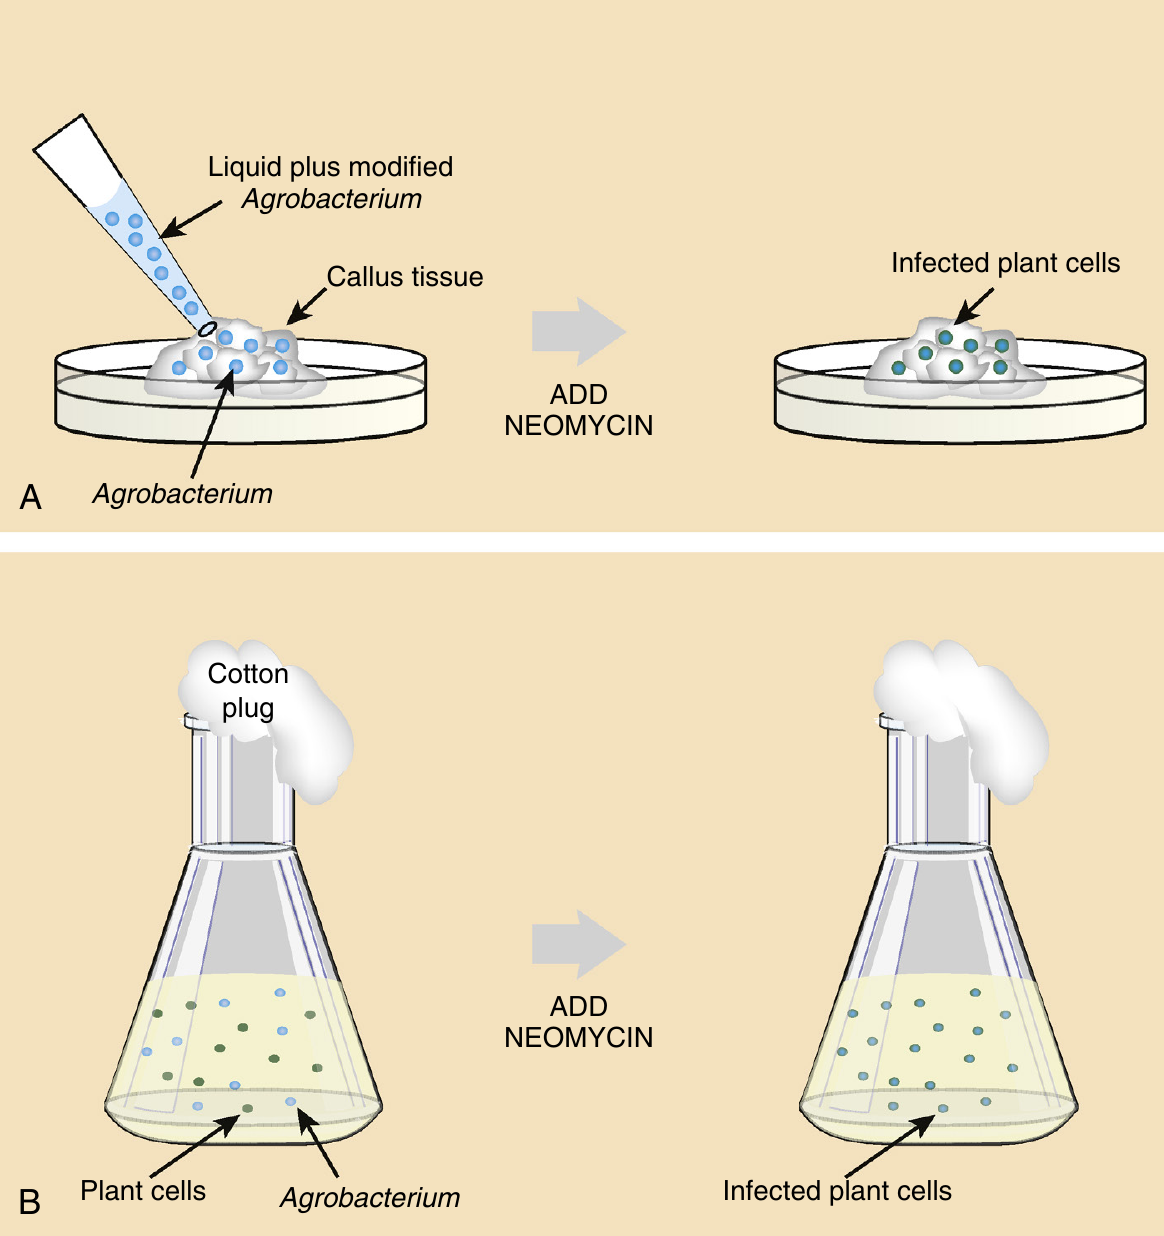
\includegraphics[width=0.35\linewidth]{../images/agrobacterium_infection_culture} \caption{\textbf{Transfer of modified Ti plasmid into a plant.} Agrobacterium carrying a Ti plasmid is added to plant tissue growing in culture. The T-DNA carries an antibiotic resistance gene (neomycin in this figure) to allow selection of successfully transformed plant cells. Both callus cultures (A) and liquid cultures (B) may be used in this procedure.}\label{fig:agrobacterium-infection-culture}
\end{figure}
\end{frame}

\begin{frame}{Agrobacterim mediated transformation in practice}
\protect\hypertarget{agrobacterim-mediated-transformation-in-practice}{}
\begin{itemize}
\tightlist
\item
  Agrobacterium is used to transfer genes of interest into plants using
  tissue culture.
\item
  Either protoplasts or a piece of callus are cultured with
  Agrobacterium harboring a Ti plasmid with modified T-DNA.
\item
  After coculture, the plant cells are harvested and incubated with the
  herbicide or antibiotic used as the selectable marker (Figure
  \ref{fig:agrobacterium-infection-culture}).
\item
  The small transgenic plants can then be screened for transgene
  expression levels.
\end{itemize}
\end{frame}

\begin{frame}{Agrobacterium mediated transformation in practice (Floral
dip method)}
\protect\hypertarget{agrobacterium-mediated-transformation-in-practice-floral-dip-method}{}
\begin{figure}
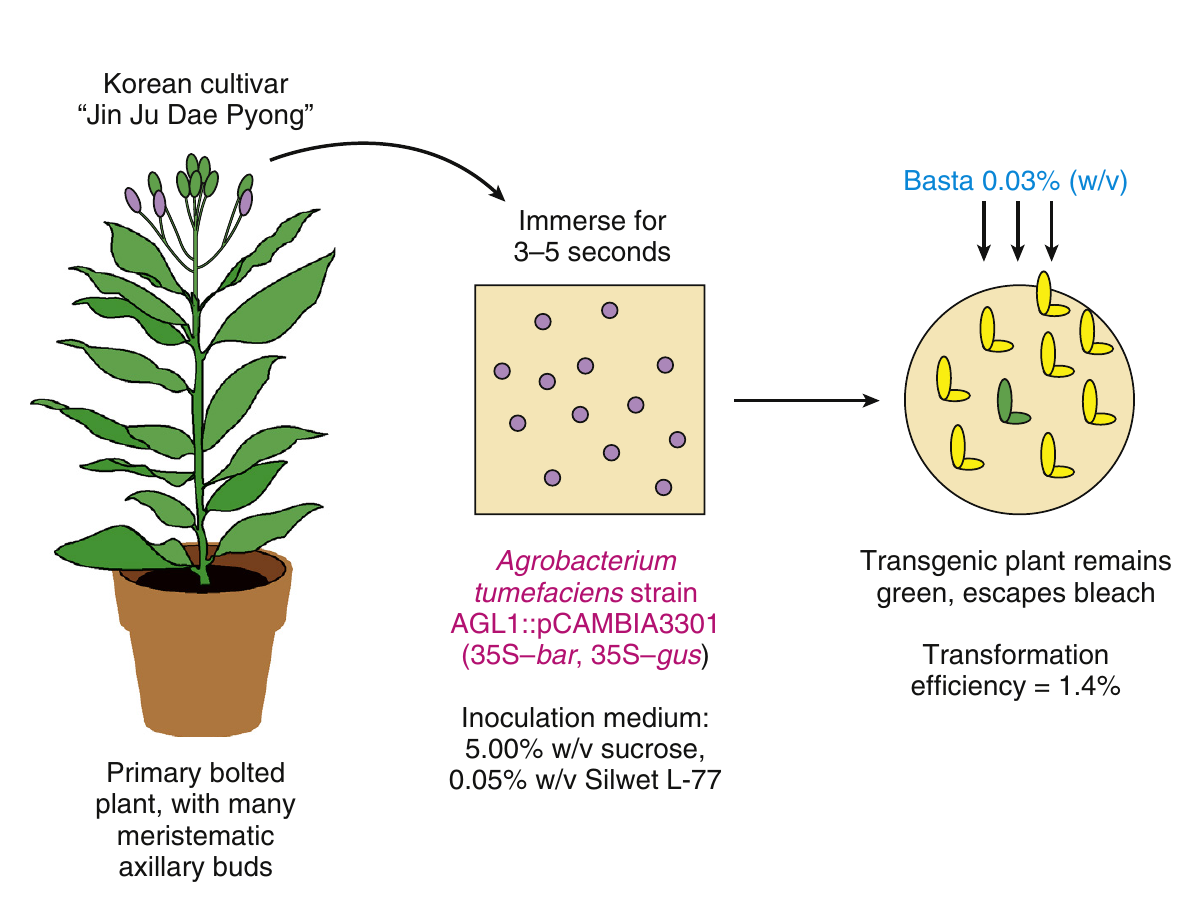
\includegraphics[width=0.45\linewidth]{../images/agrobacterium_infection_intact} \caption{\textbf{Floral dip method of plant transformation} Flower buds exposed to Agrobacterium containing modified T-DNA can result in the production of transgenic seeds. Adapted from Curtis IS (2003). The noble radish: past, present and future. Trends Plant Sci 8, 305–307.}\label{fig:agrobacterium-infection-intact}
\end{figure}
\end{frame}

\begin{frame}{Agrobacterim mediated transformation in practice (Floral
dip method)}
\protect\hypertarget{agrobacterim-mediated-transformation-in-practice-floral-dip-method}{}
\begin{itemize}
\tightlist
\item
  \emph{In planta Agrobacterium transformation} (also called floral dip
  method; Figure \ref{fig:agrobacterium-infection-intact}) has
  revolutionized plant transgenics.
\item
  The method was developed using the model plant Arabidopsis but has
  been extended to other plants, such as wheat and maize.
\item
  First, Arabidopsis plants are grown until flower buds begin to form.
  These buds are removed and allowed to regenerate for a few days. Once
  they begin to regenerate, the plants are dipped into a suspension of
  Agrobacterium containing a surfactant, which decreases surface tension
  and allows the Agrobacterium to adhere to the plant and transfer its
  T-DNA. Because the flower buds are just beginning to form, the T-DNA
  becomes part of the germline through the ovarian tissue. The plant is
  allowed to finish growing and produce seed.
\item
  Seeds are harvested and grown in selective media to find those that
  have integrated and expressed T-DNA.
\end{itemize}
\end{frame}

\hypertarget{particle-bombardment-transformation}{%
\section{Particle bombardment
transformation}\label{particle-bombardment-transformation}}

\begin{frame}{Background}
\protect\hypertarget{background-1}{}
\begin{itemize}
\tightlist
\item
  A gun blasts microscopic metal particles carrying DNA through the
  tough plant cell walls (Figure \ref{fig:gene-gun-transfer}).
\item
  Unlike Ti plasmid transfer by Agrobacterium, this technique works with
  all types of plants.
\item
  Heavy metal particles (\textasciitilde1 micrometers gold or tungsten)
  coated with DNA, accelerated toward the target tissue, and penetrate
  the cell wall to rest either adjacent to or directly in the nucleus.
\item
  Particle bombardment = Mircoprojectile bombardment = Biolistics =
  Particle acceleration = Gene gun technology
\end{itemize}
\end{frame}

\begin{frame}{Gene gune}
\protect\hypertarget{gene-gune}{}
\begin{itemize}
\tightlist
\item
  Physical method of DNA delivery
\item
  Analogy to bullet firing from a gun
\item
  Developed by John Sanford and colleagues in mid 1980s and optimized by
  Ted Klein.
\item
  Today, in most laboratories, high-pressure helium is used to generate
  the force needed to accelerate small gold particles toward the target
  tissue.
\item
  DNA is first precipitated onto the particles, which are then placed as
  a monolayer on a Mylar carrier sheet, called a macrocarrier (term is
  dubious!)
\end{itemize}
\end{frame}

\begin{frame}{Gene gun (apparatus)}
\protect\hypertarget{gene-gun-apparatus}{}
\begin{figure}
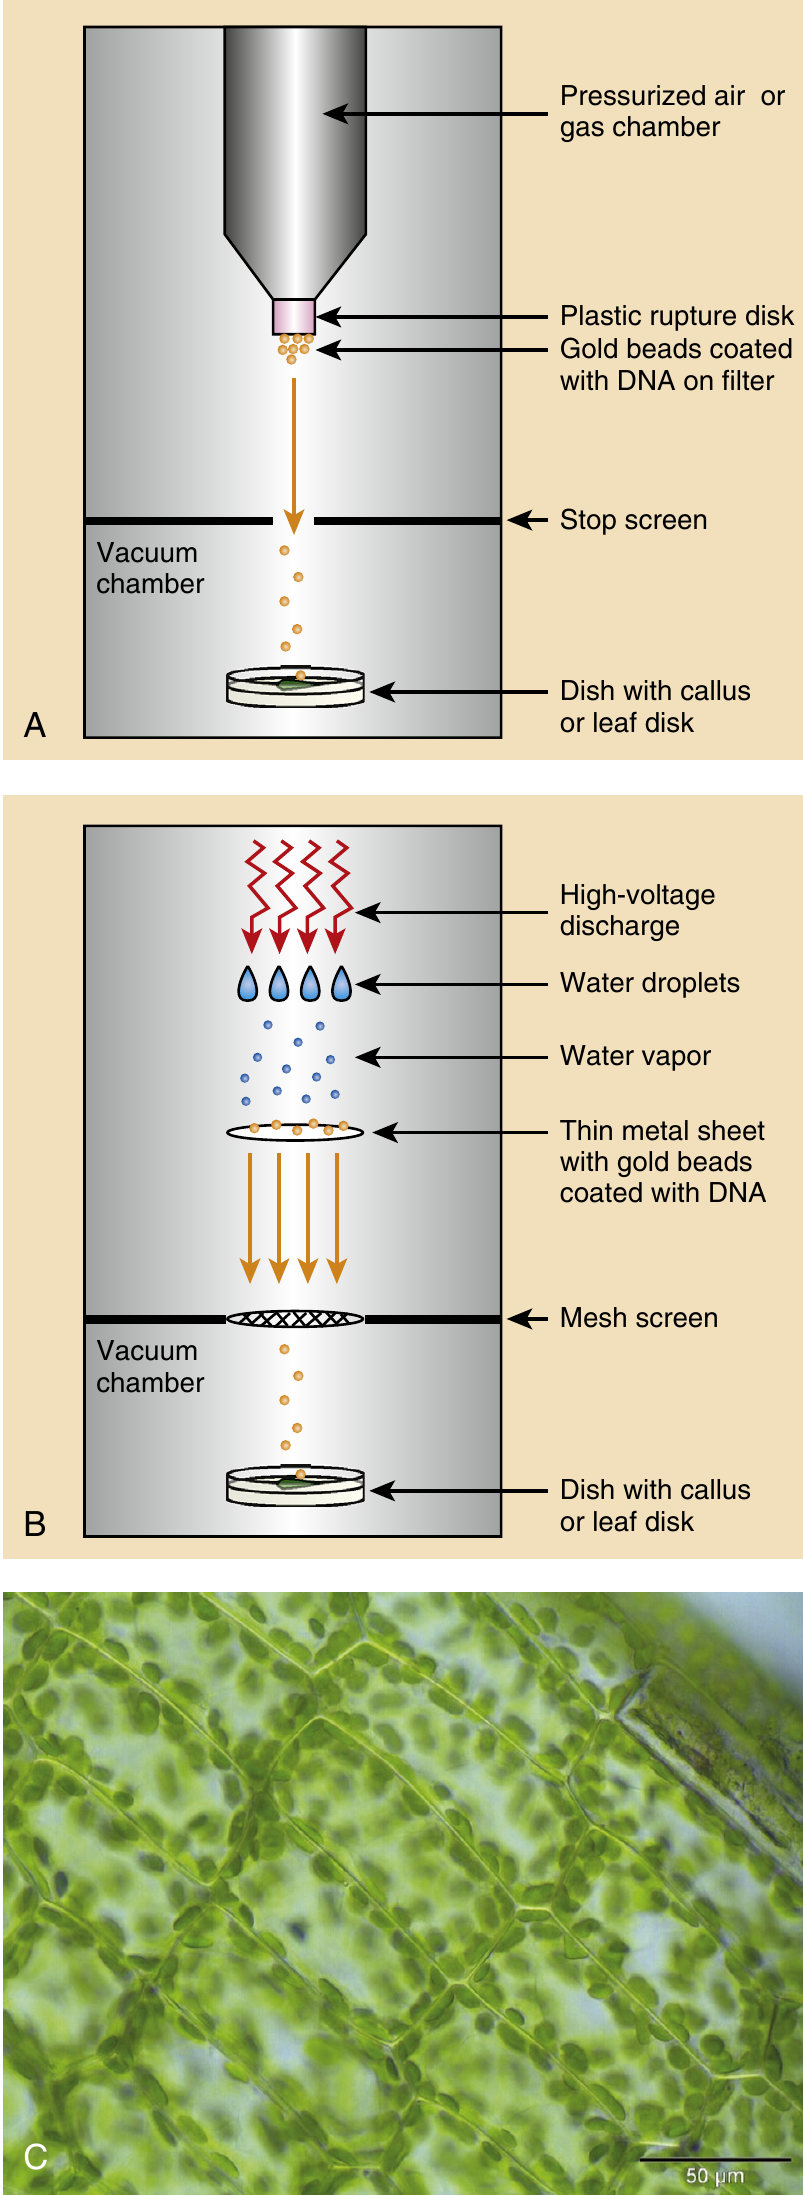
\includegraphics[width=0.16\linewidth]{../images/gene_gun_transfer} \caption{A gene gun that operates via (A) pressurized air or (B) high-voltage discharge is depicted. In both cases, the stop plate halts the projectile, and the microscopic metal particles carrying the DNA penetrate the plant tissue.}\label{fig:gene-gun-transfer}
\end{figure}
\end{frame}

\begin{frame}{Mechanism of bombardment (Pre-requisite)}
\protect\hypertarget{mechanism-of-bombardment-pre-requisite}{}
\begin{itemize}
\tightlist
\item
  DNA is first precipitated onto the particles using either calcium
  chloride or ethanol, which are commonly used for DNA precipitation.
\item
  The precipitated DNA must be able to withstand the incredible force of
  acceleration and cell wall/cytoplasm penetration and also come off the
  particles after delivery.
\item
  During bombardment, the majority of the metal particles do not find
  their target.
\end{itemize}
\end{frame}

\begin{frame}{Mechanism of bombardment (Process)}
\protect\hypertarget{mechanism-of-bombardment-process}{}
\begin{itemize}
\tightlist
\item
  A round piece of leaf tissue or a callus is isolated from the plant,
  placed on a dish, and put in a vacuum chamber.
\item
  DNA to be inserted (carrying the transgene, proper regulatory
  elements, and selectable marker) is coated on microscopic gold beads.
\item
  Beads are placed at the end of chamber. One variant of the method uses
  a blast of air or helium to drive the filter containing the gold beads
  toward the stop screen and sample.
\end{itemize}
\end{frame}

\begin{frame}{Mechanism of bombardment (Process)}
\protect\hypertarget{mechanism-of-bombardment-process-1}{}
\begin{itemize}
\tightlist
\item
  Between the bullet and plant tissue is a stop plate. Filter and gold
  beads hit this stop screen, the DNA-coated beads are thrown forward
  into the plant tissue.
\item
  An alternative method is to accelerate the beads by a strong
  electrical discharge. The high voltage vaporizes a water droplet, and
  the resulting shock wave proels a thin metal sheet covered with the
  particles at a mesh screen. The screen blocks the metal sheet but
  allows the DNA-coated particles to accelerate through into the plant
  tissue.
\item
  Advantage of this latter method is that the strength of the electrical
  discharge can be controlled; therefore, the amount of penetration into
  the tissue can be regulated.
\end{itemize}
\end{frame}

\begin{frame}{Fate of introduced DNA}
\protect\hypertarget{fate-of-introduced-dna}{}
\begin{itemize}
\tightlist
\item
  Mechanism of integration of introduced DNA to host DNA is real mess;
  many modes:

  \begin{itemize}
  \tightlist
  \item
    Single locus
  \item
    Multiple sites
  \item
    Multiple copies in single site
  \item
    Partial copies with varying orientations
  \item
    Interspersed with plant genomic DNA
  \end{itemize}
\item
  For particle bombardment, it is unclear whether the particles actually
  physically break the chromosomal DNA or merely deposit DNA in the
  proximity of the replicating parts of chromosomes.
\end{itemize}
\end{frame}

\hypertarget{detecting-the-inserted-dna}{%
\section{Detecting the inserted DNA}\label{detecting-the-inserted-dna}}

\begin{frame}{Detection system}
\protect\hypertarget{detection-system}{}
\begin{itemize}
\tightlist
\item
  Simplest of all ways is to include a selectable marker or reporter
  gene on the same segment of DNA as the transgene.

  \begin{itemize}
  \tightlist
  \item
    \emph{npt}: Encodes neomycin phosphotransferase. This enzyme confers
    neomycin resistance by attaching a phosphate group to the molecule.
    Transformed cells are directly selected with the antibiotic
    neomycin, which kills any cells that did not integrate the DNA.
  \item
    \emph{luciferase}: This enzyme emits light when provided with its
    substrate, luciferin. Key advantage is that the protein is not
    stable for long time, so the amount of active protein correlates
    with the level of gene expression at any given time. Therefore,
    \emph{luc} can be used to determine the activity of specific
    promoters.
  \end{itemize}
\end{itemize}
\end{frame}

\begin{frame}{Marker removal}
\protect\hypertarget{marker-removal}{}
\begin{itemize}
\tightlist
\item
  Removal of selectable markers (genes), which may even have unfounded
  concerns in the public is catalyzed by \emph{Cre/lox} P gene system,
  which produces Cre (``Causes recombination'') protein, that recognized
  34 base-pair DNA sequence, the \emph{\emph{loxP}} site. The Cre
  protein catalyzes recombination between two loxP sites.
\item
  The cre gene can be added to the system by cross-pollination of two
  different plants: One plant carrying the transgene plus a selectable
  marker that is flanked by two \emph{lox} P sites is crossed with
  another plant carrying the \emph{cre} gene. First, the \emph{lox} P
  pollen from the plant with the \emph{cre} gene is added to the stigma
  of the plant with the transgene. The resulting seeds are grown and
  checked for sensitivity to the selective agent (e.g., neomycin). If
  the Cre protein is present in the progeny, the selectable marker gene
  will be excised and lost during growth. This plant now has the
  transgene and the cre gene, but no longer has the gene for antibiotic
  resistance.
\end{itemize}
\end{frame}

\begin{frame}{Marker removal (procedure)}
\protect\hypertarget{marker-removal-procedure}{}
\begin{figure}
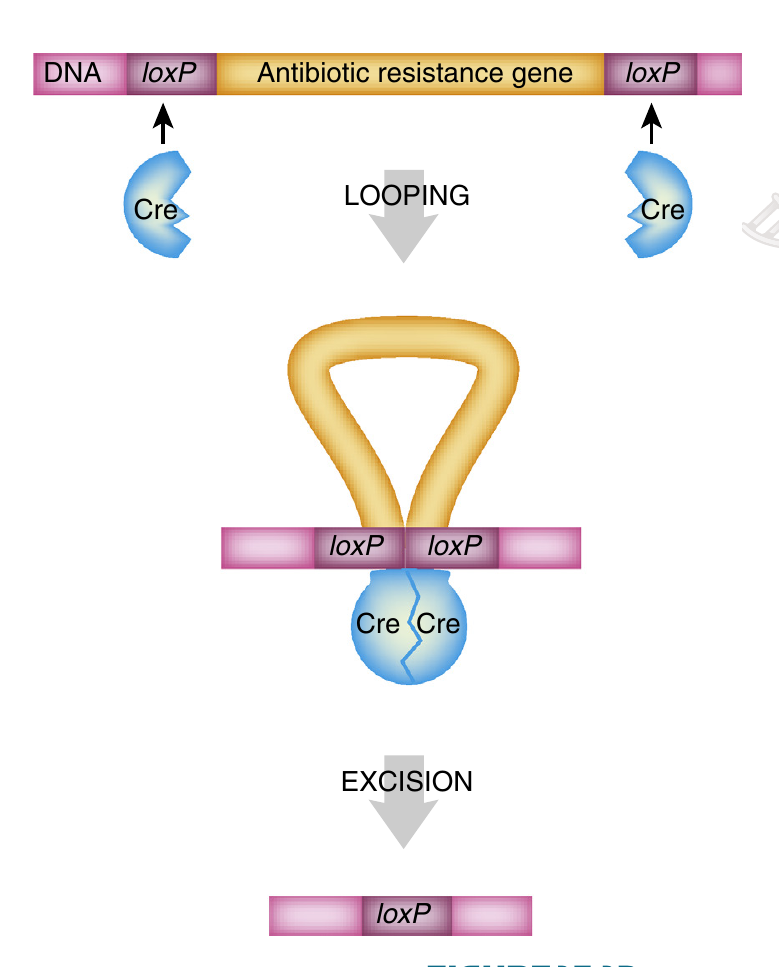
\includegraphics[width=0.35\linewidth]{../images/marker_removal} \caption{\textbf{The Cre/\textit{lox}P System of Bacteriophage P1}\newline The Cre protein binds to \textit{lox}P recognition sites in the DNA. Two nearly \textit{lox}P sites are brought together, and recombination between them eliminates the intervening DNA. A single \textit{lox}P 'scar' site remains in the target DNA molecule}\label{fig:marker-removal}
\end{figure}
\end{frame}

\hypertarget{applications}{%
\section{Applications}\label{applications}}

\begin{frame}{Engineered crops I}
\protect\hypertarget{engineered-crops-i}{}
\begin{itemize}
\tightlist
\item
  In general, to increase yield or to confer resistance to drought or
  pests
\item
  Corn lines have been modified to express

  \begin{itemize}
  \tightlist
  \item
    tolerance to either the herbicide glyphosate (RoundUp(R)) (single
    gene), or to the herbicide glufosinate-ammonium (Liberty(R));
  \item
    resistance to the pest, european corn borer (Ostrinia nubilalis)
    ECB;
  \item
    or a combination of herbicide tolerance to either glyphosate or
    glufosinate-ammonium and ECB resistance.
  \end{itemize}
\item
  Rice have been engineered with two gene pathway to enhance drought
  tolerance
\end{itemize}
\end{frame}

\begin{frame}{Engineered crops II}
\protect\hypertarget{engineered-crops-ii}{}
\begin{itemize}
\tightlist
\item
  Soybean lines have been modified to express

  \begin{itemize}
  \tightlist
  \item
    tolerance to either glyphosate, or to (Liberty),
  \item
    modified oil (high oleic acid) content.
  \end{itemize}
\item
  Cotton lines have been modified to express

  \begin{itemize}
  \tightlist
  \item
    herbicide tolerance to either glyphosate, bromoxynil or
    sulfonylurea,
  \item
    insect resistance to the pest, pink bollworm (Pectinophora
    gossypiella) PBW and tobacco budworm (Heliothis virescens) TBW.
  \item
    bromoxynil tolerance and PBW resistance.
  \end{itemize}
\end{itemize}
\end{frame}

\begin{frame}{Engineered crops III}
\protect\hypertarget{engineered-crops-iii}{}
\begin{itemize}
\tightlist
\item
  Tomato lines have been modified to

  \begin{itemize}
  \tightlist
  \item
    delay fruit ripening
  \item
    express resistance to the pests tomato pinworm, (Kieferia
    lycopersicella) TPW and tomato fruitworm (Helicoverpa zea) TFW
  \item
    express a lower polygalacturonase level which makes for a more meaty
    tomato for processing.
  \end{itemize}
\item
  Modified potato lines are

  \begin{itemize}
  \tightlist
  \item
    resistant to the Colorado Potato Beetle (Leptinotarsa decemlineata)
    CPB ,
  \item
    expresses resistance to the potato virus Y (PVY) in addition to
    being resistant to the CPB.
  \end{itemize}
\end{itemize}
\end{frame}

\begin{frame}{Transgenic technique for weed control: Glyphosate
tolerance in plants}
\protect\hypertarget{transgenic-technique-for-weed-control-glyphosate-tolerance-in-plants}{}
\footnotesize

Developing herbicide tolerance trait in the main crop is a potential
solution which can facilitate flexible use of robust non-selective and
broad spectrum herbicides. The herbicides available for killing the
weeds have two different modes of actions, selective or non-selective.
Amongst the non-selective ones, glyphosate and glufosinate are the most
extensively used herbicides. Notably, most of the herbicide-tolerant
(HT) transgenic plants have been developed so as to tolerate glyphosate
and glufosinate.

Glyphosate is environmentally friendly because it quickly breaks down to
nontoxic compounds in the soil. The glyphosate molecule is a phosphate
derivative of the amino acid glycine. Glyphosate kills plants by
blocking the synthetic pathway for the aromatic amino acids
phenylalanine, tyrosine, and tryptophan by inhibiting one particular
enzyme, EPSPS (5-enolpyruvoylshikimate-3-phosphate synthase), which is
the product of the aroA gene and localized to the chloroplast. This
target enzyme is found naturally in all plants, fungi, and bacteria, but
not in animals. Aromatic amino acids are therefore essential to the
diets of all animals, including humans, because those organisms cannot
produce them. When glyphosate is sprayed onto plants, the herbicide
penetrates the chloroplasts and binds to EPSPS, blocking the pathway for
aromatic amino acids. The plant essentially starves to death.
\end{frame}

\begin{frame}{}
\protect\hypertarget{section}{}
The development of glyphosate-resistant transgenic crops has relied on
the heterologous expression of a glyphosate-insensitive form of
\emph{epsps} obtained from either \emph{A. tumefaciens} strain CP4
(Barry et al.~1997; Padgette et al.~1995), or mutant version of maize
\emph{epsps} or chemically synthesized gene similar to \emph{epsps}
\emph{grg}23 gene of \emph{Arthrobacter globiformis}. In 1996,
glyphosate-tolerant (``Roundup Ready'') soybean harbouring
\emph{cp4epsps} gene was commercialized as the first herbicide-tolerant
transgenic crop. Most of the commercialized glyphosate-resistant crops
harbor this gene (Dill et al.~2008). Besides, a few commercialized
transgenic crops express either glyphosate oxidoreductase (GOX) encoding
gene derived from \emph{Ochrobactrum anthropi} or glyphosate
acetyltransferase (GAT) encoding gene derived from \emph{Bacillus
licheniformis}. Both of these are glyphosate-degrading enzymes which
detoxify glyphosate to non-toxic byproducts.
\end{frame}

\begin{frame}{}
\protect\hypertarget{section-1}{}
\begin{figure}
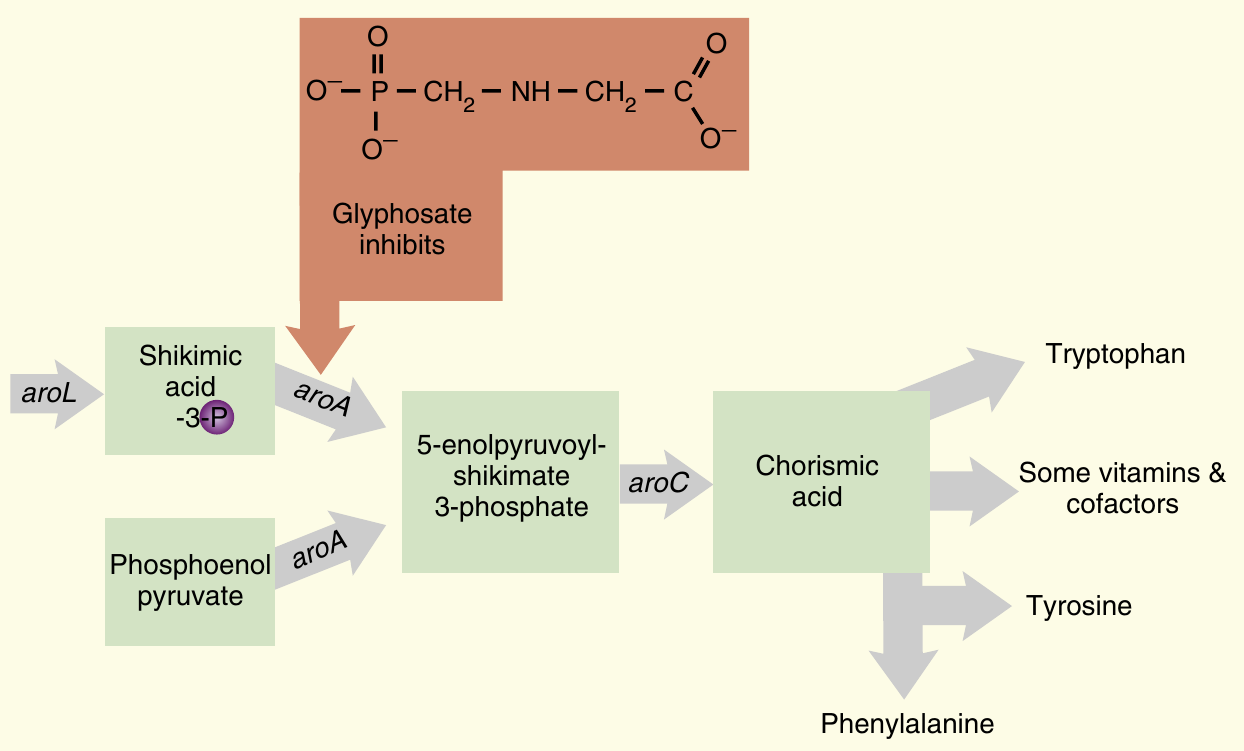
\includegraphics[width=0.5\linewidth]{../images/epsps_pathway_plants} \caption{EPSPS pathway in plants}\label{fig:glyphosate-tolerance}
\end{figure}
\end{frame}

\begin{frame}{Transgenic technique for protection against insect:
Bt-toxin technology}
\protect\hypertarget{transgenic-technique-for-protection-against-insect-bt-toxin-technology}{}
\begin{figure}
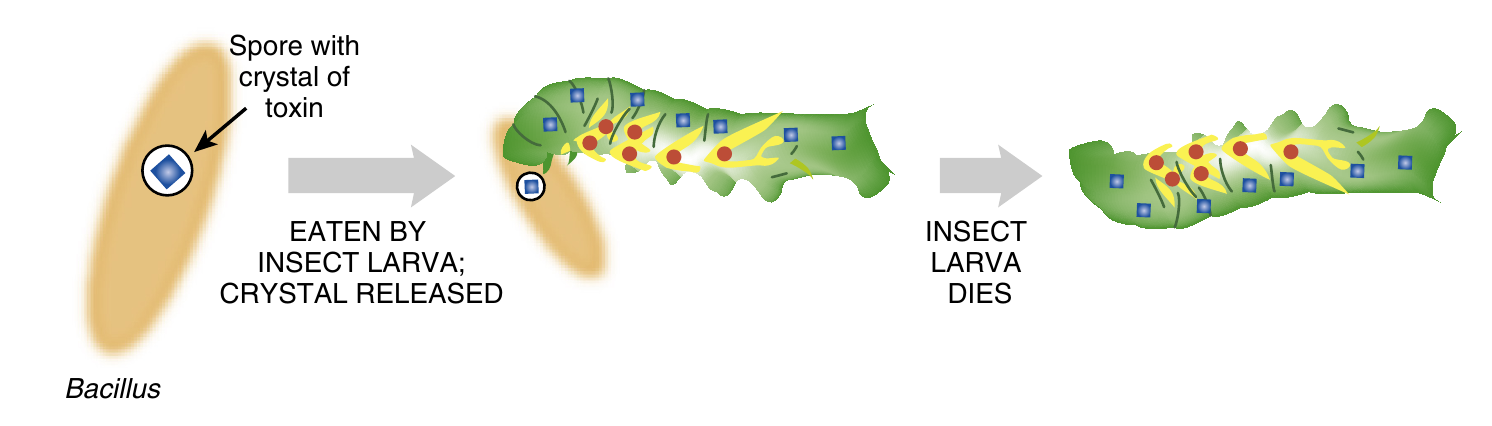
\includegraphics[width=0.6\linewidth]{../images/bt_toxin_mechanism} \caption{\textbf{Insect Larvae Are Killed by Bt Toxin}Bacterial spores of Bacillus are found on food eaten by caterpillars. The crystalline protein is released by digestion of the spore, and its breakdown produces a toxin that kills the insect larvae.}\label{fig:bt-toxin-mechanism}
\end{figure}
\end{frame}

\begin{frame}{Transgenic technique for protection against insect: Insect
avoidance technique}
\protect\hypertarget{transgenic-technique-for-protection-against-insect-insect-avoidance-technique}{}
\begin{figure}
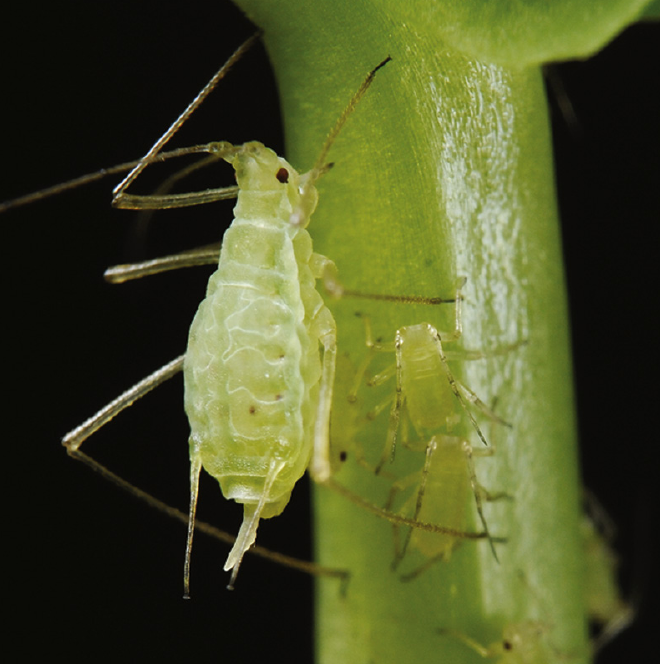
\includegraphics[width=0.4\linewidth]{../images/aphid_avoidance} \caption{Aphids feed on sap, but plants expressing (E) -$\beta$ farnesene can scare them away. Photo courtesy of Shipher Wu and Geeway Lin, National Taiwan University.}\label{fig:aphid-avoidance}
\end{figure}
\end{frame}

\hypertarget{bibliography}{%
\section{Bibliography}\label{bibliography}}

\begin{frame}{Further study}
\protect\hypertarget{further-study}{}
Also see: Rajasekaran, Jacks, and Finley (2002), Clark and Pazdernik
(2016)
\end{frame}

\begin{frame}{References}
\protect\hypertarget{references}{}
\hypertarget{refs}{}
\begin{cslreferences}
\leavevmode\hypertarget{ref-clark2016biotechnology}{}%
Clark, David P, and Nanette J Pazdernik. 2016. \emph{Biotechnology}.
Elsevier.

\leavevmode\hypertarget{ref-rajasekaran2002crop}{}%
Rajasekaran, Kanniah, Thomas J Jacks, and John W Finley. 2002.
\emph{Crop Biotechnology}. ACS Publications.

\leavevmode\hypertarget{ref-stachel1986genetic}{}%
Stachel, Scott E, and Eugene W Nester. 1986. ``The Genetic and
Transcriptional Organization of the Vir Region of the A6 Ti Plasmid of
Agrobacterium Tumefaciens.'' \emph{The EMBO Journal} 5 (7): 1445--54.
\end{cslreferences}
\end{frame}

\end{document}
